\documentclass{article}

\documentclass[preview,12pt]{article}
\usepackage{amsmath}
\usepackage{gensymb}
\usepackage{ragged2e}
\usepackage{geometry}
\usepackage{graphicx}
\usepackage{caption}
\usepackage{subcaption}
\usepackage{pdfpages}

\geometry{letterpaper, margin=1in}

\begin{document}

\begin{titlepage}
    \vspace*{\fill}
    \begin{center}
        \LARGE \textit{"Laser Absorption Spectroscopy-Measurement of Methane Concentration in a Jet"}
    \end{center}
    \begin{center}
       \large Josh Coffey
    \end{center}
    \begin{center}
        \large University of Cincinnati
    \end{center}
    \begin{center}
        \large November 2019
    \end{center}
        \vspace*{\fill}
\end{titlepage}

\begin{center}
    \section*{Introduction}
\end{center}
$$$$
\indent This lab had students measure the concentration of methane in a methane/air mixture by using Laser Induced Florescence.  They used a helium-neon laser with a wavelength of 3.39 $\mu$m, which resulted in a linearly polarized beam in the Infrared range of the electromagnetic spectrum. The lab involved moving a Centuro burner so that the airstream coming out of the top of the burner moves through a laser beam.  The beam power was read by a detector on the opposite side of the burner and this power was converted to voltage, and this value was measured and displayed by an oscilloscope.  Various data measurements were taken at different points in the airstream. \newline
\indent This data was then used to calculate the concentration of methane in the airstream.  Using the resulting value and a program that runs a 3 point Abel deconvolution the field distribution is calculated.  Using this value, the concentration was able to be calculated.

$$$$

\begin{center}
    \subsection*{Laser Absorption Spectroscopy}
\end{center}
$$$$
\indent Laser absorption Spectroscopy is a line of sight method of measuring the concentration of a particular molecule within a medium.  For example, in this lab, the concentration of methane was measured in a jet of air and methane.  \newline
\indent The principle behind laser absorption spectroscopy is that when a laser beam with a frequency that is similar to the transition frequency of the medium passes through that medium, some of the photons are absorbed and the amount of power of the laser that can be detected on the other side of the medium can be translated into useful information about the medium.  This method compares the incident power to the power that is measured, $\frac{I}{I_0}$ to measure the amount of the laser that was absorbed.  \newline
\indent Once the ratio of powers is known, Beer-Lambert's law is used to find the concentration of the absorbing species.
$$\frac{I}{I_0}=10^{-\epsilon c l}$$
where $\epsilon$ is the decadic molar extinction coefficient that is distinct for each species, $l$ is the absorption path length, and $c$ is the concentration of the absorbing species and is given by 
$$c=\frac{P_{pt}}{R_uT}$$
where $P_{pt}$ is the species partial pressure, $R_u$ is the universal gas constant, and T is the temperature. \newline
\indent Then, using 3 point abel deconvolution, which begins with the projected field input
$$P(x)=-ln\left(\frac{I}{I_0}\right)=2\int_x^R\frac{f(r)rdr}{(r^2-x^2)^{.5}}$$
and transforms this value to the field distribution.
$$f(r)=c\epsilon '$$
as can be seen in figure 1, where c is the concentration and $\epsilon '=\epsilon\textrm{ }ln 10$. \newline
\indent Note that this method of measurement gives an average temperature and concentration of the medium, and is less accurate for non uniform temperatures and concentrations.  However, if either temperature or concentration are known, as in the isothermal case, the other can be calculated.  Temperature can be found using the absorption profile and the integral of $\Gamma(v)$.

\begin{figure}[h]
    \centering
    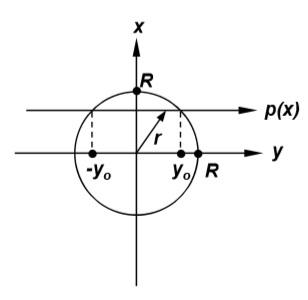
\includegraphics[width=.6\textwidth]{3pointAbelDeconvolution.PNG}
    \caption*{\footnotesize{Figure 1: 3 Point Abel Deconvolution  (Lee, Absorption Lab, Fall 2019)}}
\end{figure}


$$$$

\begin{center}
    \subsection*{Experimental Setup and Procedure}
\end{center}
$$$$
\indent As mentioned above, the laser used in this experiment is an infrared, helium-neon laser with a wavelength of 3.39 $\mu$m.  The laser is able to output a minimum power of 2 milliwatts and a maximum power of 5 milliwatts.  This produces a beam with a diameter of 2.02 millimeters and a divergence of 2.13 milliradians.  The beam travels to the focusing lens, which tightens the beam.  This lens transmits 50\% of the laser beams power.  The beam then passes through the medium that is being released through the Centuro burner.  For this experiment, there is a methane - air mixture surrounded by a flow of air which serves to keep the "flame" steady. \newline 
\indent After passing over the Centuro burner, the beam reaches the detector, which has two filters in front of the detector.  The first filter is a neutral density filter that transmits 10\% of the beam and is immediately followed by a narrow bandpass filter that transmits 70\% of the remaining beam.  The beam finally reaches the detector, which has a diameter of 2 millimeters. The detector is cooled in order to minimize the effects of dark current on the final reading, which converts the detected beam power to a current. \newline
\indent This current is run through a transimpedence amplifier, which converts the current output by the detector into a voltage that is then displayed by an oscilloscope. This value is estimated by first calculating the power that is read by the detector.  This calculation begins as follows:
$$2.0\textrm{mW}\cdot0.5\cdot0.1\cdot0.7=70\mu W$$
This will be the estimated value that is read by the detector.  The detector then converts this value to a current, with an known efficiency of 70\%.  The amplifier then converts to a voltage with a gain of $2.5x10^4$.  This gives an output voltage of 1.23 Volts.\newline
\indent To set up the system, the laser aligned with the focusing lens and the detector using traverses that control the heights of the lens and detector. In addition, the lens is able to be rotated.  Once the system is aligned, which is determined by when voltage read on the oscilloscope is maximized, the lens and detector are locked into place using a magnetic base.  This system is represented in figure 2. \newline
\begin{figure}[h]
    \centering
    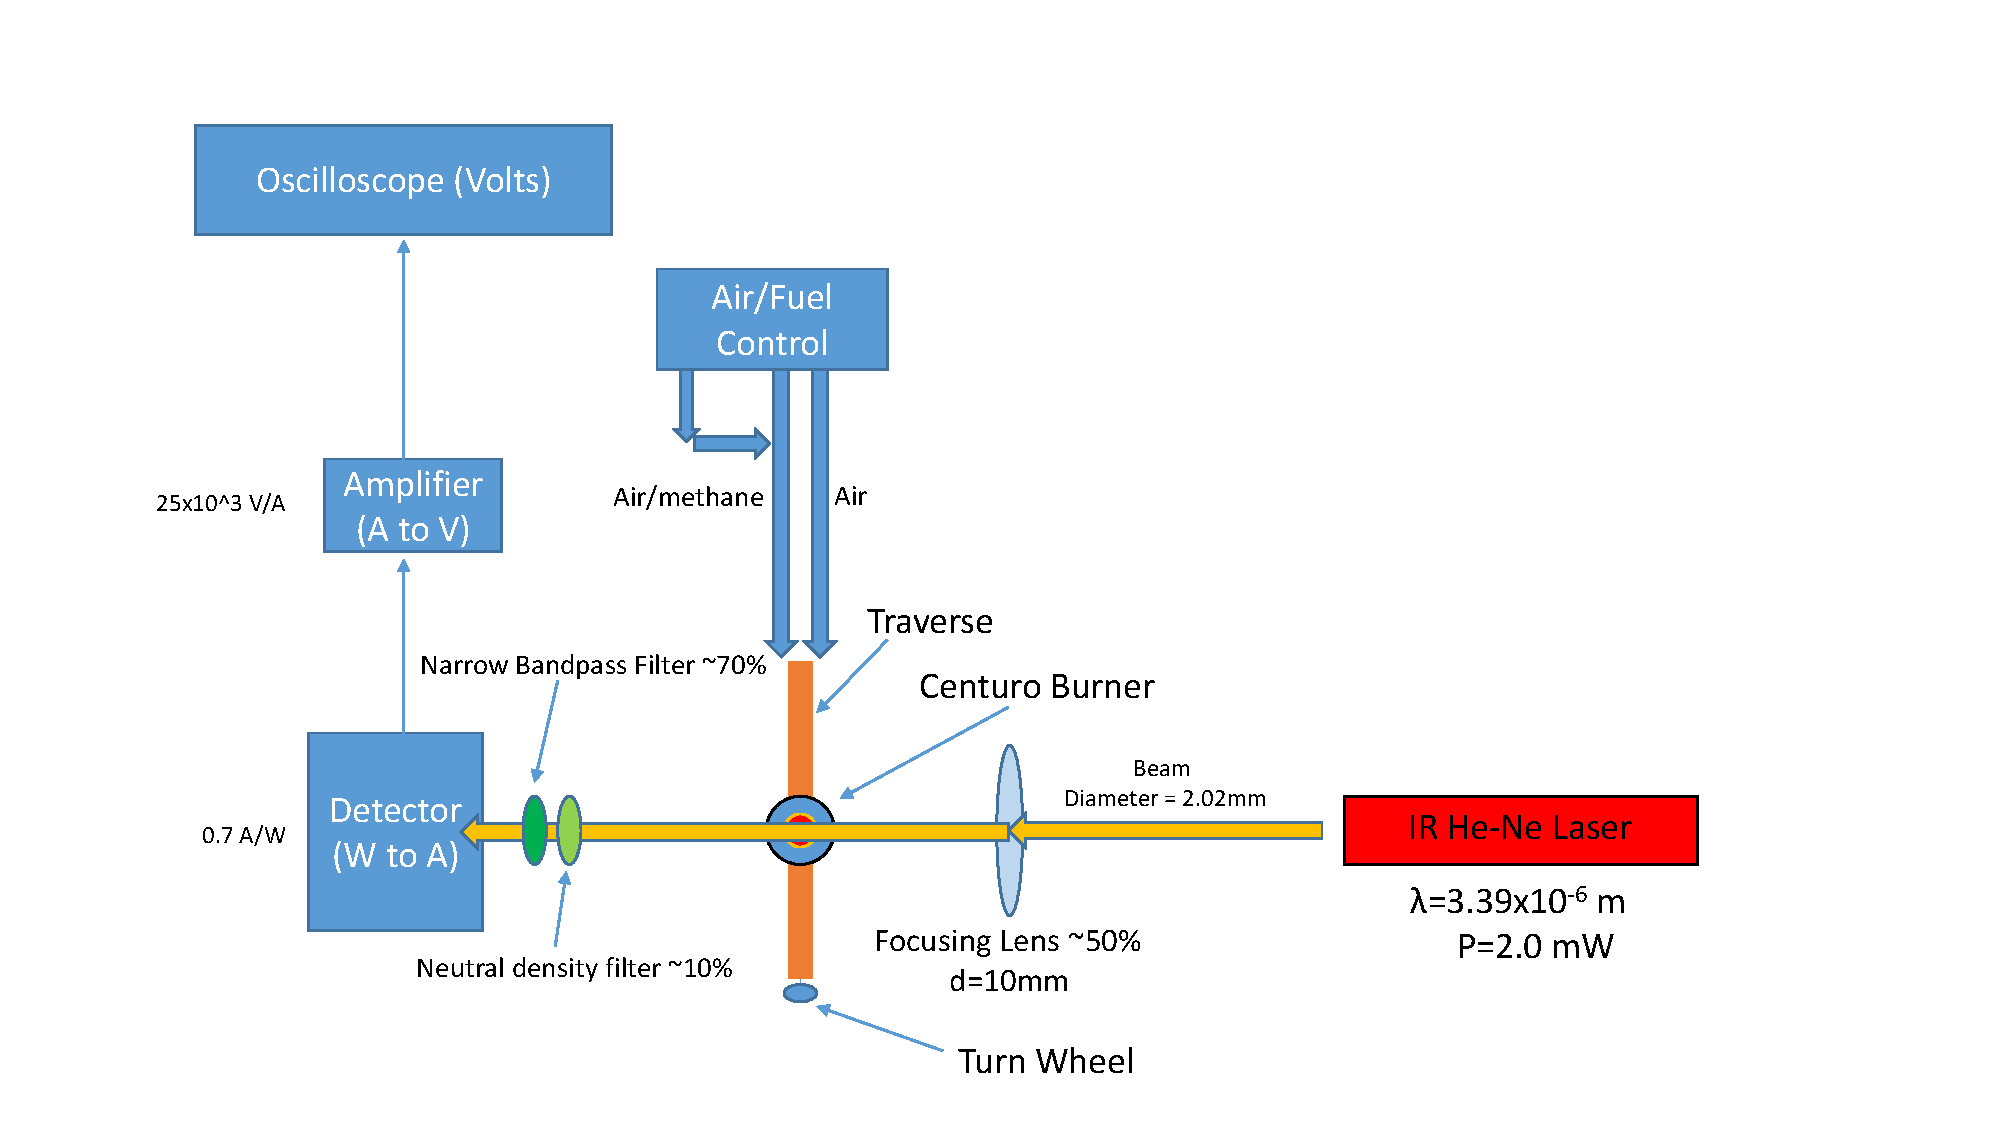
\includegraphics[width=\textwidth]{Lab1Diagram.pdf}
    \caption*{\footnotesize{Figure 2: Experimental Setup}}
\end{figure}
\indent To carry out the experiment, the methane-air/air flows is run to the Centuro burner, without a flame.  The burner is attached to a traverse that has a wheel that moves the burner 1/20th of an inch for each turn. Starting with the burner away from the burner, the wheel is turned until the airflow is touching the laser beam.  At this point, the voltage is read from the oscilloscope.  Then the turn wheel is turned once to move the burner further into the laser beam and the voltage is read from the oscilloscope.  After approximately four turns, the air is turned off to check that the beam has not changed.  This process is repeated until the voltage reading is minimized, which represents the center of the stream being released by the burner.  Lastly, a few extra readings were taken to ensure that the center was reached.\newline
\indent This process is conducted for a Reynolds number of 5000 and 7500.  The Reynolds number is varied by changing the flow rates of the air and methane/air mixes. At 5000, $\dot{m}_{air}$=0.000787624 $\frac{kg}{s}$ and $\dot{m}_{fuel}$=0.000421781$\frac{kg}{s}$.   At 7500, $\dot{m}_{air}$=0.0.001181436 $\frac{kg}{s}$ and $\dot{m}_{fuel}$=0.000632671$\frac{kg}{s}$.  The ambient pressure and temperature were estimated to be 1 atm and 70\degree F respectively.\newline
\indent Once all the data was taken, the center of the jet was taken as the point at which the value of $\frac{I}{I_0}$ was minimized.  Using this value and calculating the approximate jet radius using the fact that one turn of the wheel was Then, taking 15 data points chosen by dividing the jet radius by the number of desired data points, i.e. 15, and sequencing up by one "step," so that the data is evenly spaced from the outside of the jet to the center, the projected field is calculated. Then, these values of the field are run through a 3-step abel deconvolution which results in the field distribution. \newline
\indent Using this value, and known values of $\epsilon=85000$ and $\epsilon '=195719.7329$, the concentration as mol/cm$^3$ was calculated.  Then, this data was used to create several plots: $\frac{I}{I_0}$ vs vol\% of methane and C$_\textrm{deconvoluted}$ vs R.  The 
\newpage

\begin{center}
    \subsection*{Data Analysis}
\end{center}
$$$$
\begin{center}
    \subsection*{Estimating Jet Radius}
\end{center}
To estimate the jet radius, as mentioned above, the location at which I$_{transmitted}$ was minimized was chosen from the collected data.  This was taken to be the center of the jet and then the number of turns to the outside of the jet were counted.  The outside of the jet was determined to be when the transmitted power did not change after a turn.  Because each turn was known to be $\frac{1}{20}$ of an inch, the radius of the jet was able to be calculated and was found to be 1.93816756 cm for Re = 5000 and 1.58269915 cm for Re = 7500.

\begin{center}
    \subsection*{Similarity of Concentration Field with Dowling and Dimotakis}
\end{center}

Dowling and Dimotakis found looked at concentration as a specially similar property.  This means that their value of concentration was normalized so that they were independent of Reynolds's number, while the concentrations of this experiment were dependent on reynolds number which meant that it was a generally similar property.  In addition, the scales of Dowling and Dimotakis' graph was different than the one produced in this experiment due to their graph being the mean concentration of several different experiments. 

\begin{center}
    \subsection*{Discussion}
\end{center}
\indent This data is what was expected, with a concentration that is roughly gaussian in shape.  This implies that the methane is more concentrated in the center of the jet with a drop-off in concentration as measurements move radially outward.  This is also the expected shape of the jet overall. \newline

\indent Some sources of error include: dark current, destructive or constructive interference from ambient light sources, the laser beam not being perfectly aligned with the detector, and the assumptions that were made in the calculations.  Cooling the detector reduced the amount of dark current, but may have not completely prevented it from affecting the measurements.  The laser beam was aligned with the detector by hand, and was locked into place when the voltage on the oscilloscope seemed maximized.  However, this leaves the possibility that the system may not have been perfectly aligned with the detector, and a more precise alignment method may provide more accurate results. Ambient light should not have made a large impact on the results due to the polarization of the beam, but it is possible that some of the laser beam was slightly affected by the ambient light that was similarly oriented.  This could be reduced by reducing the amount of ambient light, but this would make it difficult to conduct the experiment.  The largest potential source of error is the assumptions that were made.  These include: assuming that the power out of the laser was the minimum possible power, assuming standard conditions for ambient pressure and temperature, and assuming that the known transmission amounts through the different components of the system were perfectly accurate.  These assumptions could all be removed by conducting a thorough review and measurement of all parts of the system. \newline

\indent This experiment assumes that the mixture is isothermal.  However, it is possible that the jet may not be isothermal if, for example, a flame was added.  In this case, one way to still measure the species concentration using only absorption spectroscopy would be to find the temperature from the curve fit to the Voigt profile and use that temperature to calculate the concentration.  This would need to be repeated for many different data points, making absorption spectroscopy less than ideal for non isothermal situations.  
\newpage
\begin{center}
    \section*{References}
\end{center}


Dowling, David R., and Paul E. Dimotakis. “Similarity of the Concentration Field of Gas-Phase Turbulent Jets.” \textit{Journal of Fluid Mechanics}, vol. 218, 1990, pp. 109–141., doi:10.1017/S0022112090000945.
\newline
$$$$
Dasch, Cameron J. "One-Dimensional tomography: A comparison of Abel, Onion-Peeling, and Filtered Back Projection Methods." \textit{Optical Society of America}, 1991
\newline
$$$$
Eckbreth, A.C., "Laser Diagnostics for Combustion Temperature and Species", 2nd ed., 1996, Gordon and Breach Publishers
\newpage

\begin{center}
    \section*{Appendix}
\end{center}

\begin{center}
    \subsubsection*{C$_{deconvoluted}$ vs R}
\end{center}
\begin{figure}[h]
    \centering
    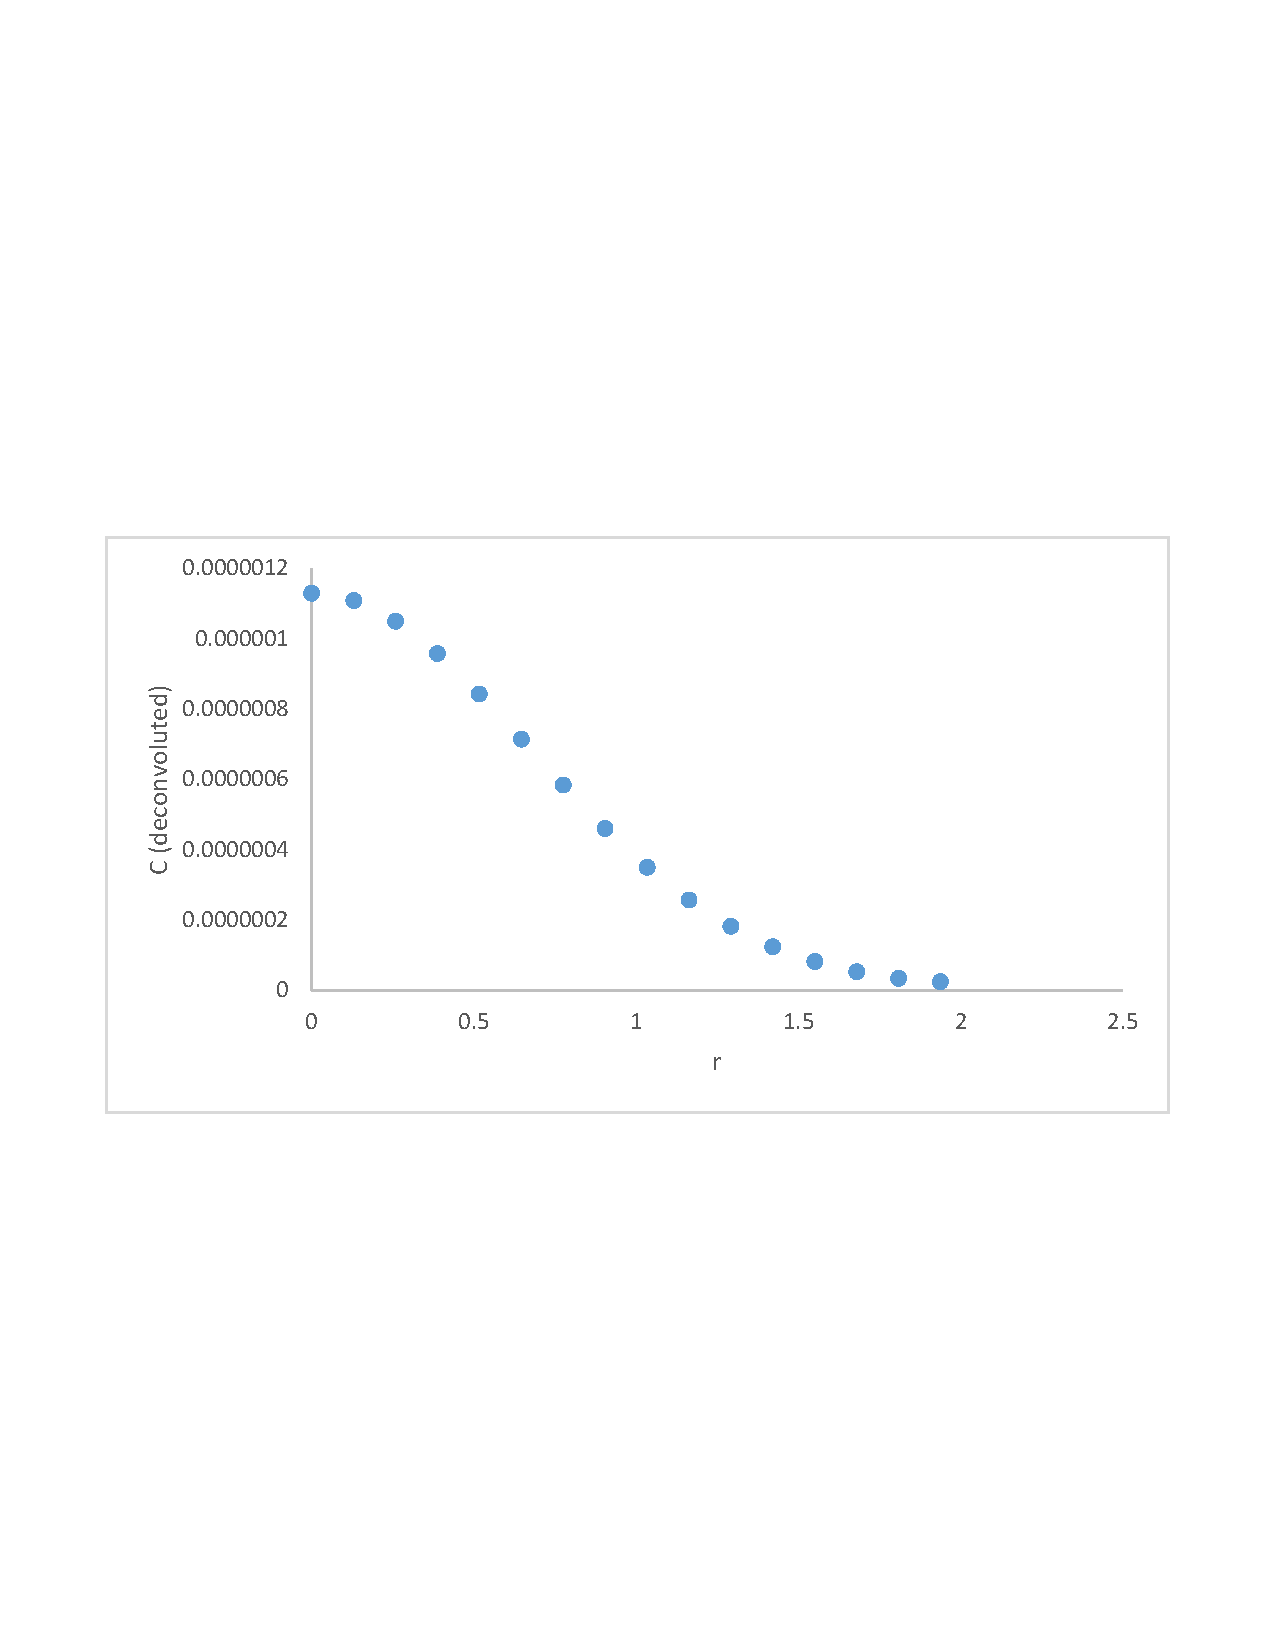
\includegraphics[width=.7\textwidth]{Lab1_CvsR_5000.png}
    \caption*{\footnotesize{Figure 3: C$_{deconvoluted}$ vs R at Re=5000}}
\end{figure}
\begin{figure}[h]
    \centering
    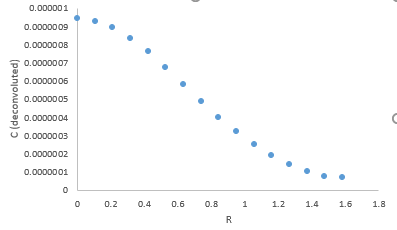
\includegraphics[width=.7\textwidth]{Lab1_CvsR_7500.png}
    \caption*{\footnotesize{Figure 4: C$_{deconvoluted}$ vs R at Re=7500}}
\end{figure}
\newpage
\begin{center}
    \subsubsection*{I/I$_0$ vs \% Volume}
\end{center}
\begin{figure}[h]
    \centering
    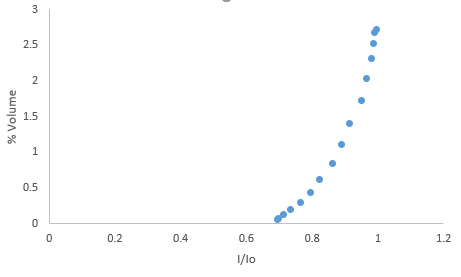
\includegraphics[width=.7\textwidth]{LAB1_5000_IoVSVol.PNG}
    \caption*{\footnotesize{Figure 5: I/I$_0$ vs \% Volume at Re=5000}}
\end{figure}
\begin{figure}[h]
    \centering
    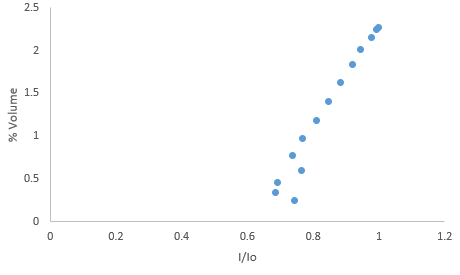
\includegraphics[width=.7\textwidth]{LAB1_7500_IoVSVol.PNG}
    \caption*{\footnotesize{Figure 6: I/I$_0$ vs \% Volume at Re=7500}}
\end{figure}







\end{document}
